% Goldilocks --- PRX Quantum article (Phase 6 REVTeX conversion).
% Source of truth for submission edits. The markdown under paper/prose/
% is the frozen first draft; do not dual-maintain.
% Do not flatten the polarity: peaks exist; they never win.
% Exactness is free; advantage is not.
% Do not load amsthm: REVTeX 4.2 already defines \proof.
\documentclass[aps,prx,reprint,floatfix,amsmath,amssymb,amsfonts]{revtex4-2}

\usepackage{graphicx}
\usepackage{bm}

\newtheorem{theorem}{Theorem}
\newtheorem{lemma}{Lemma}
% REVTeX 4.2 conflicts with amsthm; this bundle does not ship \proof.
% Manual environment: optional title, closed by a qed box.
\newenvironment{proof}[1][Proof]{%
  \par\medskip\noindent\textit{#1.}\ignorespaces
}{%
  \unskip\nobreak\hfill$\square$\par\medskip
}

\begin{document}

\title{Noise cannot help quantum-enhanced MCMC: exactness is free, advantage is not}

\author{Darth Kuvius}
\affiliation{TODO: affiliation}
\email[]{TODO: corresponding-author email}

\date{\today}

\begin{abstract}
Quantum-walk Metropolis proposals give an exactly correct Markov-chain
sampler whenever the proposal is symmetric, without evaluating proposal
probabilities. We classify the noise channels that preserve that free
lunch: every transpose-closed Kraus set --- dephasing in any real basis,
depolarizing noise, and equal-rate raising and lowering --- yields a
symmetric proposal at any strength. The condition extends to Lindblad
semigroups with a real-symmetric walk Hamiltonian by a time-reversed
Dyson unravelling. Amplitude damping ($T_1$) is the unique realistic
violator; a device that keeps the evaluation-free Metropolis ratio on a
damped proposal runs naive Metropolis rather than Hastings, with a
proved per-step total-variation bound of order the symmetry defect and a
(typically loose) stationary envelope. Exactness is therefore free for
the noise that dominates today's devices. Advantage is not. Intermediate
dephasing can accelerate the walk's own mixing --- the interior optimum
is a known property of decohered walks, and we give an exact
window-averaged telegraph solution that isolates the even-moment
coherences time randomization cannot kill. Those Goldilocks peaks never
lift the sampler above the envelope of the coherent quench and trivial
classical kernels on Gibbs targets. A pre-registered test on fifty
random Ising, Sherrington--Kirkpatrick, and random-field instances finds
the envelope law in forty-nine cells, with one disclosed $+1.17\%$
instance-specific exception; in every cell where the coherent quench
already wins, dephasing erodes the win. The Metropolis filter is why
environment-assisted transport does not transfer to sampling:
delocalization broadens proposal energy, and the filter rejects the
spread. Noise costs nothing and buys nothing.
\end{abstract}

\maketitle

\section{Introduction}

Markov-chain Monte Carlo (MCMC) draws samples from a target $\pi$ on a
set too large to enumerate by proposing a move and accepting or
rejecting it. The quality of the sampler is the quality of the
proposals. Layden \emph{et al.}~\cite{Layden2023} showed that a short
coherent quantum quench, used only as a proposal inside an otherwise
classical Metropolis--Hastings (MH) kernel, can suggest long-range,
energy-preserving jumps that a local classical kernel misses, and that
the construction remains \emph{exactly} correct whenever the proposal is
symmetric --- no evaluation of the proposal probabilities is required.
On hardware they observed that the sampler stayed accurate under
realistic noise. That robustness was treated as a nuisance property,
stated in their Supplemental Material as a symmetry-on-average
condition, and left unclassified.

A different literature makes noise look like a resource. In
environment-assisted quantum transport (ENAQT), a moderate dephasing
rate delocalizes an excitation that pure coherent dynamics would trap,
and a large rate freezes it~\cite{Rebentrost2009,LloydMohseni2011}. The
same ``Goldilocks'' interior optimum appears in the mixing time of
decohered quantum walks on the line, the cycle, and the
hypercube~\cite{KendonTregenna2003,Fedichkin2006,AlagicRussell2005,Drezgich2009}
--- a phenomenon we cite as known, and return to in Secs.~\ref{sec:advantage}
and~\ref{sec:related}. The tempting conjecture for today's noisy devices
is that a tuned dephasing rate should likewise help a quantum-walk
\emph{Metropolis proposal}: noise would cost nothing (exactness already
survived it in Layden's experiment) and might buy mixing (ENAQT and the
walk literature say it can). We call that conjecture noise-as-resource,
and we tested it as three hypotheses: H1, a Goldilocks peak in sampling
efficiency; H2, a stable matching $\gamma^\ast/\Delta$ across targets;
H3, a hardware walk that beats its own zero-idle configuration because
native noise already sits near $\gamma^\ast$.

The answer is two-sided, and we do not flatten it. Realistic decoherence
splits cleanly. Every transpose-closed noise channel --- dephasing in
any real basis, depolarizing noise, infinite-temperature relaxation ---
preserves the evaluation-free exactness of the sampler at \emph{any}
strength. $T_1$ amplitude damping is the unique realistic channel that
does not, and the bias it induces when a device keeps the free-lunch
Metropolis ratio is bounded. That is the positive half: exactness is
free. The negative half is not ``noise never helps mixing.'' Noise
\emph{does} create Goldilocks peaks. In a solvable corner the
window-averaged gap rises from $0.5$ to $0.97$; in the field, twenty of
fifty random cells show an interior peak. Those peaks never lift the
sampler above the envelope of the coherent quench and the trivial
classical kernels. Wherever the quantum proposal already has an
advantage, dephasing erodes it; wherever dephasing helps the walk, a
classical kernel was already better. Advantage is not free, and H1--H3
die in that form. Noise costs nothing and buys nothing.

We make four contributions.

\begin{enumerate}
\item \emph{A characterization of exactness-preserving noise}
(Theorems~\ref{thm:tc} and~\ref{thm:lindblad}). Transpose-closed Kraus
sets give symmetric proposals; the condition extends to Lindblad
semigroups with real-symmetric $H$ and transpose-closed jumps via a
time-reversed Dyson unravelling. Layden's SM stated the
symmetry-on-average condition; we classify the channels that satisfy it.
Certification places every transpose-closed class at defect
$\le 1.2\times 10^{-14}$ and the violators at $\ge 3.5\times 10^{-2}$.

\item \emph{A quantitative $T_1$ budget}
(Theorems~\ref{thm:perstep} and~\ref{thm:stationary}). A device that
ignores the $q$-ratio on a damped proposal runs naive Metropolis, not
Hastings. The per-step total-variation distance is at most
$\varepsilon(1/\pi_{\min}-1)$; the stationary distance is at most that
times $\pi_{\min}^{-1/2}/\delta$. Measured TV is $O(\varepsilon)$; the
gap envelope is guaranteed and typically loose by $10^6$--$10^{21}$. The
working device requirement is $\varepsilon\lesssim\eta$, or else
estimate the $q$-ratio.

\item \emph{A refutation of gap-monotonicity, a solvable corner, and the
envelope law} (Sec.~\ref{sec:advantage}). Gap-monotonicity in $\gamma$
is false. The window-averaged telegraph solution plus the odd/even-moment
mechanism explain \emph{why} noise can help mixing, and embed that known
phenomenon in an exact MH sampler. The envelope law --- noise never
beats $\max(\text{coherent},\,\text{classical})$ --- is pre-registered
and holds in $49/50$ random cells, with one disclosed $+1.17\%$
instance-specific exception. In advantage cells, dephasing erodes beyond
$\gamma\approx 0.03\Delta$. Orfi and Sels already rule out a worst-case
unital speedup~\cite{OrfiSels2024}; our law is the per-instance,
family-wide complement.

\item \emph{A reusable benchmarking protocol} (Sec.~\ref{sec:protocol}).
Kernels never see target log-probabilities; ESS per step and per second
are both reported; split-$\hat R\le 1.05$ gates frozen chains; kill
criteria are written before data; negative results are reported at full
strength. The protocol killed H1 on the G01 pilot and then caught the
overreach of conjecture v1, forcing the G05 pre-registration.
\end{enumerate}

Section~\ref{sec:setup} fixes notation. Section~\ref{sec:exactness} is
exactness. Section~\ref{sec:advantage} is advantage.
Section~\ref{sec:mechanism} is the mechanism that stops ENAQT from
transferring to sampling --- the Metropolis filter, not a failure of
delocalization. Section~\ref{sec:outlook} flags a forward-looking
predictor, energy concentration, as a conjecture and not a result of
this paper. Related work is collected in Sec.~\ref{sec:related} rather
than here; the short version is that we are the first channel-level
classification of exactness for noisy walk proposals, and the first
embedding of decohered-walk mixing results in an exact MH sampler with
Gibbs targets.

For quantum-walk Metropolis proposals we (i) characterize exactly which
noise channels preserve evaluation-free exactness (transpose-closed
Kraus sets --- dephasing in any real basis, depolarizing, equal-rate
$\sigma^\pm$ --- at any strength, with $T_1$ the unique realistic bias
channel), and (ii) establish the envelope law: tuned dephasing, although
it genuinely accelerates the walk's own mixing as known since Kendon and
Tregenna~\cite{KendonTregenna2003}, never lifts the sampler's efficiency
above the envelope of the coherent quench and trivial classical kernels
on Gibbs targets. Exactness is free, advantage is not.

\section{Setup}
\label{sec:setup}

We sample a target $\pi$ on the hypercube $\{0,1\}^n$. The
Metropolis--Hastings (MH) kernel built from a proposal $q(\cdot|x)$ is
\begin{equation}
  P(y|x)
  =
  q(y|x)\, a(y,x)
  \qquad (y \neq x),
\end{equation}
with $P(x|x) = 1 - \sum_{y \neq x} P(y|x)$ and acceptance
\begin{equation}
  a(y,x)
  =
  \min\Bigl(1,\;
  \frac{\pi(y)\, q(x|y)}{\pi(x)\, q(y|x)}\Bigr).
\end{equation}
If $q$ is symmetric, $q(y|x) = q(x|y)$, the proposal ratio cancels and
the acceptance collapses to the evaluation-free Metropolis ratio
$\min(1,\pi(y)/\pi(x))$. That is the free lunch of Layden
\emph{et al.}~\cite{Layden2023}: a quantum proposal that never has to be
evaluated still yields an exactly correct sampler, provided symmetry
holds.

The family we study is a \emph{dephased quantum walk} used only as a
proposal. The walk Hamiltonian is real symmetric,
\begin{equation}
  H
  =
  (1-\alpha)\, \mathrm{diag}(E)
  +
  \alpha \sum_{i=1}^{n} X_i,
\end{equation}
with mixer weight $\alpha \in (0,1]$ and $E$ the classical energy whose
Gibbs distribution is $\pi$. The generator is the Lindbladian
\begin{gather}
  \mathcal{L}(\rho)
  =
  -i[H,\rho]
  +
  \gamma \sum_{i=1}^{n} \mathcal{D}[Z_i](\rho),
  \nonumber\\
  \mathcal{D}[A](\rho)
  =
  A\rho A^\dagger - \tfrac12 \{A^\dagger A,\rho\}.
\end{gather}
A single proposal from $x$ is a computational-basis measurement of
$\mathcal{E}_t(|x\rangle\langle x|)$,
\begin{equation}
  q_t(y|x)
  =
  \langle y|\, \mathcal{E}_t(|x\rangle\langle x|) \,|y\rangle,
  \qquad
  \mathcal{E}_t = e^{t\mathcal{L}}.
\end{equation}
Following Layden, we average $t$ uniformly over a fixed window (in units
of the spectral width $\Delta$ of $H$; the G01/G05 window is
$t\Delta \in [2,12]$). The window-averaged proposal is written
$q_\gamma$. Two limits are named: $\gamma = 0$ is the coherent quench of
Layden \emph{et al.}; $\gamma \to \infty$ is a Zeno freeze in the
computational basis, recovered in practice as a lazy classical kernel.

Two equivalent realizations of $\mathcal{E}_t$ are used throughout. At
$n \le 6$ we exponentiate the dense superoperator (or apply it sparsely
on a time grid) and read the proposal matrix exactly. At larger $n$ the
same channel is sampled by a quantum-trajectory unravelling: one shot is
one Poisson record of phase kicks, one trajectory, and one proposal.
That unravelling is also the circuit recipe (stochastic Hamiltonian
phase kicks, or a collision scheme with ancilla resets). Because the
jump statistics of computational-basis dephasing are state-independent,
the trajectory sampler never consults $\pi$.

Classical baselines, used only as competitors and never as ingredients
of the walk, are Metropolized single-flip (Hamming-1) and uniform-flip
(the complete graph). Efficiency is reported as the MH spectral gap
$\delta(P) = 1-|\lambda_2(P)|$ wherever the $2^n \times 2^n$ kernel can
be built, and as effective sample size per step and per second on gated
MCMC runs (Sec.~\ref{sec:protocol}). Nothing in this section is a claim
about noise; the claims begin when $\gamma > 0$ or when the channel is
replaced by a different physical noise model.

\section{Exactness is free}
\label{sec:exactness}

The free lunch requires
$q(y|x) = \langle y|\, \mathcal{E}(|x\rangle\langle x|) \,|y\rangle$ to
be symmetric in $(x,y)$. Layden \emph{et al.} already state the
operational condition in their Supplemental Material: errors are
harmless ``provided such errors do not break the $Q(s'|s)=Q(s|s')$
symmetry on average.'' Our contribution is the channel-level
\emph{classification} of which physical noise satisfies that condition,
at any strength, together with a quantitative bound for the one
realistic violator.

The proposal basis $\{|x\rangle\}$ is the computational basis
throughout; transposes are taken in this basis.

\subsection{Transpose-closed channels}

\begin{theorem}[Transpose-closed Kraus sets]
\label{thm:tc}
Let $\mathcal{E}(\rho) = \sum_a K_a \rho K_a^\dagger$ admit a Kraus
representation $\{K_a\}_{a=1}^{m}$ that is closed under transposition
up to unitary remixing,
\begin{equation}
  K_a^{\mathsf T}
  =
  \sum_b u_{ab}\, K_b
  \qquad
  \text{for some unitary } u \in \mathrm{U}(m).
  \tag{TC}
\end{equation}
Then $q(y|x) = q(x|y)$ for all $x,y$.
\end{theorem}

\begin{proof}
For real basis vectors,
$\langle x|K_a|y\rangle = \langle y|K_a^{\mathsf T}|x\rangle$. Hence
\begin{align}
  q(x|y)
  &=
  \sum_a \bigl|\langle x|K_a|y\rangle\bigr|^2
  =
  \sum_a \bigl|\langle y|K_a^{\mathsf T}|x\rangle\bigr|^2
  \nonumber\\
  &=
  \sum_a \Bigl|\sum_b u_{ab}\, \langle y|K_b|x\rangle\Bigr|^2
  =
  \sum_b \bigl|\langle y|K_b|x\rangle\bigr|^2
  =
  q(y|x),
\end{align}
the last-but-one step because $u$ preserves the $\ell^2$-norm of the
amplitude vector $v_b = \langle y|K_b|x\rangle$.
\end{proof}

Condition (TC) says that $\{K_a^{\mathsf T}\}$ is \emph{also} a Kraus
representation of $\mathcal{E}$. The set $\{K_a^{\mathsf T}\}$ always
represents the map $\Theta \circ \mathcal{E}^\star \circ \Theta$, where
$\Theta$ is transposition and $\mathcal{E}^\star$ is the Heisenberg
adjoint (Kraus $\{K_a^\dagger\}$). Two Kraus sets represent the same
channel if and only if they are unitarily related, so (TC) is exactly
the representation-independent identity
\begin{equation}
  \mathcal{E}
  =
  \Theta \circ \mathcal{E}^\star \circ \Theta.
  \tag{TC$'$}
\end{equation}
A channel either has a transpose-closed Kraus set or it does not.

Unitary remixing preserves $\sum_a A_a^\dagger A_a$, so (TC) implies
$\sum_a (K_a^{\mathsf T})^\dagger (K_a^{\mathsf T}) = \sum_a K_a^\dagger K_a = I$,
hence $\mathcal{E}(I) = I$: every transpose-closed channel is unital. A
symmetric proposal is column-stochastic and symmetric, hence doubly
stochastic, and $\sum_x q(y|x) = \langle y|\mathcal{E}(I)|y\rangle$, so
\begin{equation}
  \mathrm{diag}\bigl(\mathcal{E}(I)\bigr) = 1
  \quad
  \text{is necessary for symmetry.}
  \tag{N}
\end{equation}
Non-unital noise with a non-flat diagonal of $\mathcal{E}(I)$ --- any
channel that relaxes toward a preferred state, including
finite-temperature amplitude damping --- breaks symmetry before any
interference argument is needed.

Condition (TC) is sufficient, not necessary. Symmetry constrains only
the diagonal-to-diagonal block of $\mathcal{E}$ (the transition matrix
$P = P^{\mathsf T}$), while (TC$'$) constrains the whole superoperator.
Contrived channels can be symmetric without (TC). The honest statement,
and the one we make, is structural: every physically arising symmetric
case below satisfies (TC), and the physically arising violator
(finite-$T$ damping) already fails the weaker necessary condition (N).

\subsection{Lindblad semigroups}

\begin{theorem}[Lindblad semigroups]
\label{thm:lindblad}
Let $\mathcal{L}(\rho) = -i[H,\rho] + \sum_j \gamma_j \mathcal{D}[L_j](\rho)$.
Suppose
(i) $H = H^{\mathsf T}$ is real symmetric;
(ii) the weighted jump set is transpose-closed: there is a permutation
$j \mapsto j'$ with $L_j^{\mathsf T} = e^{i\phi_j} L_{j'}$ and
$\gamma_j = \gamma_{j'}$;
(iii) $\sum_j \gamma_j L_j^\dagger L_j$ is real symmetric, or
equivalently the effective non-Hermitian Hamiltonian
$H_{\mathrm{eff}} = H - (i/2)\sum_j \gamma_j L_j^\dagger L_j$ satisfies
$H_{\mathrm{eff}}^{\mathsf T} = H_{\mathrm{eff}}$.
Then $\mathcal{E}_t = e^{t\mathcal{L}}$ satisfies (TC) for every
$t \ge 0$, hence $q_t(y|x) = q_t(x|y)$ for all $t$.
\end{theorem}

\begin{proof}[Proof (time-reversed Dyson unravelling)]
The time-ordered decomposition of $e^{t\mathcal{L}}$ is the continuous
Kraus family indexed by jump records
$\omega = (m;\, t_1 < \cdots < t_m;\, j_1,\ldots,j_m)$,
\begin{gather}
  K_\omega
  =
  G(t-t_m)\, \sqrt{\gamma_{j_m}} L_{j_m} \cdots \sqrt{\gamma_{j_1}} L_{j_1}\, G(t_1),
  \nonumber\\
  G(s) = e^{-i H_{\mathrm{eff}} s},
\end{gather}
with
$e^{t\mathcal{L}}(\rho) = \sum_m \int dt_1\cdots dt_m \sum_{j_1\ldots j_m} K_\omega \rho K_\omega^\dagger$.
Transposition reverses operator order. By (iii), $G(s)^{\mathsf T} = G(s)$;
by (ii), each $L_j^{\mathsf T}$ is a phase times $L_{j'}$ at the same
rate. Hence
\begin{gather}
  K_\omega^{\mathsf T}
  =
  e^{i\Phi(\omega)}\, K_{\tilde\omega},
  \nonumber\\
  \tilde\omega
  =
  (m;\, t-t_m < \cdots < t-t_1;\, j_m',\ldots,j_1'),
\end{gather}
the time-reversed, transpose-relabelled record. The map
$\omega \mapsto \tilde\omega$ is a measure-preserving involution of the
index set (Lebesgue measure on the time-simplex is invariant under
$s \mapsto t-s$; the rate weights match by (ii)), and phases are killed
by $|\cdot|^2$. The Kraus family is therefore transpose-closed and
Theorem~\ref{thm:tc} applies.
\end{proof}

Condition (iii) is implied by (i)+(ii) when the jumps are real (up to
phase) and normal ($L^{\mathsf T}L = LL^{\mathsf T}$); every row of
Table~\ref{tab:channels} has normal jumps. Time-reversal is
load-bearing: a product of symmetric operators is not symmetric,
$(AB)^{\mathsf T} = BA$, so ``each instant is symmetric'' does not give
``the semigroup is symmetric.'' Naive composition fails; the Dyson
involution is the mechanism. Symmetry survives convex mixtures ---
including Layden's random $t$-window and a random $\gamma$ --- and
time-reversal-symmetric compositions, but not arbitrary composition of
two different symmetric channels.

\subsection{Which physical noise is free}

Table~\ref{tab:channels} and Fig.~\ref{fig:symmetry} collect the
classification. Computational-basis dephasing ($Z_i$ jumps, any rate),
dephasing in \emph{any} real basis (jumps $A = VDV^{\mathsf T}$ with $V$
real orthogonal), depolarizing and arbitrary Pauli-jump noise, and
infinite-temperature relaxation ($\sigma^-$ and $\sigma^+$ at equal
rates) all satisfy (TC). Amplitude damping ($\sigma^-$ only) and
finite-$T$ relaxation at unequal rates fail (N) and break symmetry.

The last two rows are the sharp pair: the same jump operators, and the
matching condition $\gamma_+ = \gamma_-$ is exactly what flips symmetry
on. Noise that drives toward the maximally mixed state preserves the
free lunch; noise that knows a preferred state ($T_1$ relaxation toward
$|0\rangle$) breaks it.

Numerical certification pins every row. The worst defect over all
transpose-closed channels is $1.2\times 10^{-14}$ across
$n\in\{4,5\}$ ($n=6$ for computational dephasing),
$\gamma/\Delta \in \{0.1,1,10\}$, and $t\Delta \in \{0.5,2,8\}$. Both
negative controls --- amplitude damping, and unequal-rate $\sigma^\pm$
with $\gamma_+ = \gamma_-/4$ --- break at defect
$\ge 3.5\times 10^{-2}$. The certified-file maximum for amplitude
damping is $0.352$ (at $\kappa = 0.1\Delta$, $t\Delta \le 8$); an older
grid's $0.55$ is not in the current file and is not used here.

\begin{table*}
\caption{\label{tab:channels}
Channel classes, transpose closure, and certified symmetry defect
$\max_{x,y}|q(y|x)-q(x|y)|$.}
\begin{ruledtabular}
\begin{tabular}{llll}
Noise channel & Transpose closure & Symmetric? & Certified defect \\
Computational-basis dephasing, jumps $Z_i$, any rate
  & $Z_i^{\mathsf T} = Z_i$ & yes & $\le 3.3\times 10^{-16}$ \\
Dephasing in any real basis, $A = VDV^{\mathsf T}$
  & $A^{\mathsf T} = A$ & yes & $\le 1.3\times 10^{-14}$ \\
Depolarizing / Pauli-jump noise (rates arbitrary)
  & $X^{\mathsf T}=X$, $Z^{\mathsf T}=Z$, $Y^{\mathsf T}=-Y$
  & yes & $\le 10^{-15}$ \\
Infinite-$T$ relaxation (equal-rate $\sigma^\pm$)
  & $(\sigma^-)^{\mathsf T}=\sigma^+$, rates matched
  & yes & $\le 10^{-15}$ \\
Amplitude damping / unequal-rate $\sigma^\pm$
  & $(\sigma^-)^{\mathsf T}=\sigma^+\notin$ set; fails (N)
  & no & $\ge 3.5\times 10^{-2}$ (file max $0.352$) \\
\end{tabular}
\end{ruledtabular}
\end{table*}

\begin{figure}
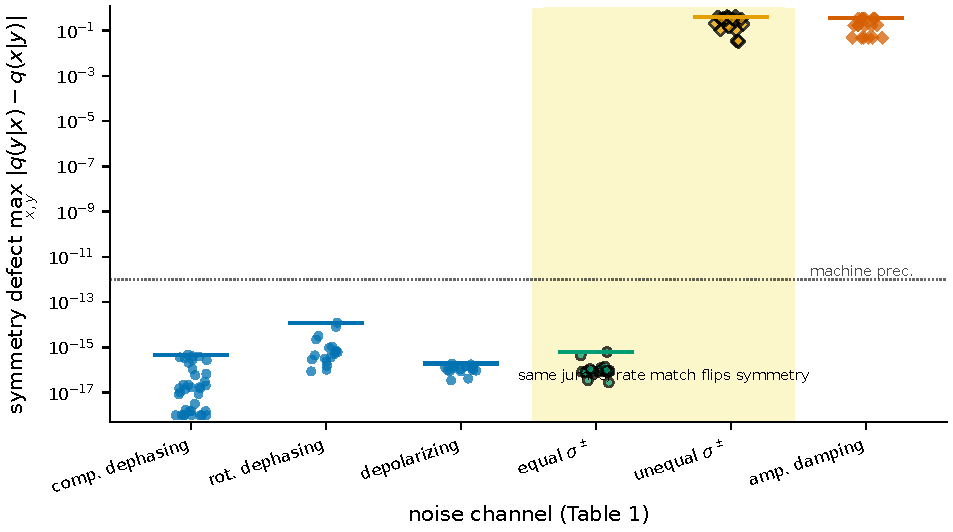
\includegraphics[width=\linewidth]{figures/fig1_symmetry.pdf}
\caption{\label{fig:symmetry}
Symmetry defect versus channel class on a log scale. Transpose-closed
classes sit at machine precision; amplitude damping and unequal-rate
$\sigma^\pm$ sit between $3.5\times 10^{-2}$ and $0.352$. The
equal/unequal $\sigma^\pm$ pair is highlighted: the same jumps, and only
the rate-matching condition, decide exactness.}
\end{figure}

Device noise is, to a first accounting, dephasing ($T_\varphi$) plus
amplitude damping ($T_1$) plus gate depolarizing plus coherent
overrotation (real $H$ errors). By Table~\ref{tab:channels}, $T_\varphi$
at any rate, depolarizing gate noise, and real-Hamiltonian
miscalibration are all exactness-free. \emph{$T_1$ relaxation is the
unique realistic bias channel.} A hardware claim has to bound or
estimate only the damping component; everything else rides free. That is
the formal content of the robustness Layden \emph{et al.} observed
empirically.

\subsection{$T_1$ bias: naive Metropolis versus Hastings}

A device that keeps the free-lunch Metropolis ratio on a $\kappa$-damped
proposal $\tilde q$ is \emph{not} running the exact Hastings kernel.
Write $P_H$ for Hastings on $\tilde q$ (acceptance includes the
$q$-ratio; stationary distribution exactly $\pi$) and $P_M$ for naive
Metropolis (acceptance $\min(1,\pi(y)/\pi(x))$; stationary
$\tilde\pi \neq \pi$ in general). The theorem is not
$\|\tilde q_{\kappa=0} - \tilde q_\kappa\|$; that is a proposal-TV
statement and is not controlled by the symmetry defect. Write
$\varepsilon = \max_{x,y} |\tilde q(y|x) - \tilde q(x|y)|$ for the
symmetry defect.

\begin{theorem}[Per-step TV]
\label{thm:perstep}
For every state $x$,
\begin{align}
  \bigl\| P_M(\cdot|x) - P_H(\cdot|x) \bigr\|_{\mathrm{TV}}
  &\le
  \sum_{y\neq x} \frac{\pi(y)}{\pi(x)}\, \bigl|\tilde q(y|x) - \tilde q(x|y)\bigr|
  \nonumber\\
  &\le
  \varepsilon \bigl(1/\pi(x) - 1\bigr).
\end{align}
Uniformly over $x$,
\begin{equation}
  \|P_M - P_H\|_{\mathrm{TV},\infty}
  \le
  \varepsilon \bigl(1/\pi_{\min} - 1\bigr),
\end{equation}
where $\pi_{\min} = \min_x \pi(x)$ and
$\|\cdot\|_{\mathrm{TV},\infty} = \max_x \|\cdot(\cdot|x)\|_{\mathrm{TV}}$.
\end{theorem}

\begin{proof}
For $y\neq x$,
$|P_M(y|x)-P_H(y|x)| = \tilde q(y|x)\, |\min(1,r)-\min(1,r\rho)|$ with
$r=\pi(y)/\pi(x)$ and $\rho = \tilde q(x|y)/\tilde q(y|x)$
($\rho:=1$ if $\tilde q(y|x)=0$). The elementary inequality
$|\min(1,a)-\min(1,b)|\le |a-b|$ gives
$|\min(1,r)-\min(1,r\rho)| \le r|1-\rho|$, hence
\begin{equation}
  |\Delta P(y|x)|
  \le
  \tilde q(y|x)\, r\, |1-\rho|
  =
  \frac{\pi(y)}{\pi(x)}\, \bigl|\tilde q(y|x)-\tilde q(x|y)\bigr|.
\end{equation}
The diagonal difference equals $-\sum_{y\neq x}\Delta P(y|x)$, so
$|\Delta P(x|x)| \le \sum_{y\neq x}|\Delta P(y|x)|$. Therefore
\begin{align}
  \|\Delta P(\cdot|x)\|_{\mathrm{TV}}
  &=
  \tfrac12 \sum_y |\Delta P(y|x)|
  \nonumber\\
  &\le
  \sum_{y\neq x} |\Delta P(y|x)|
  \le
  \varepsilon\bigl(1/\pi(x)-1\bigr).
\end{align}
\end{proof}

If $\varepsilon=0$ --- every transpose-closed channel in
Table~\ref{tab:channels} --- then $P_M=P_H$ and there is no free-lunch
bias. $T_1$ remains the unique realistic channel that can make
$\varepsilon>0$. Hastings on a $T_1$-damped proposal is still exact; the
cost is evaluating the $q$-ratio.

\begin{theorem}[Stationary TV]
\label{thm:stationary}
Let $\delta = \delta(P_H) = 1-|\lambda_2(P_H)|$ be the spectral gap of
the exact Hastings kernel. Then
\begin{align}
  \|\tilde\pi - \pi\|_{\mathrm{TV}}
  &\le
  \frac{1}{\delta}\, \pi_{\min}^{-1/2}\, \|P_M-P_H\|_{\mathrm{TV},\infty}
  \nonumber\\
  &\le
  \varepsilon \bigl(1/\pi_{\min}-1\bigr)\, \pi_{\min}^{-1/2}/\delta.
\end{align}
\end{theorem}

\begin{proof}
Stationarity gives $\tilde\pi P_M = \tilde\pi$ and $\pi P_H = \pi$, so
$(\tilde\pi-\pi)(I-P_H) = \tilde\pi(P_M-P_H) =: \nu$. Work in
$L^2(\pi)$ via densities $f = d\mu/d\pi$. $P_H$ is reversible, hence
self-adjoint on densities in $L^2(\pi)$; on the mean-zero subspace,
$\|(I-P_H)^{-1}\|_{L^2(\pi)} \le 1/\delta$. Both $\tilde\pi-\pi$ and
$\nu$ are mean-zero. With $f = d(\tilde\pi-\pi)/d\pi$ and
$g = d\nu/d\pi$,
\begin{equation}
  \|\tilde\pi-\pi\|_{\mathrm{TV}}
  =
  \tfrac12 \|f\|_{L^1(\pi)}
  \le
  \tfrac12 \|f\|_{L^2(\pi)}
  \le
  \tfrac{1}{2\delta}\|g\|_{L^2(\pi)}.
\end{equation}
Then
$\|g\|_{L^2(\pi)}^2 = \sum_y \nu(y)^2/\pi(y) \le \pi_{\min}^{-1}(\sum_y|\nu(y)|)^2$,
so $\|g\|_{L^2(\pi)} \le \pi_{\min}^{-1/2}\cdot 2\|\nu\|_{\mathrm{TV}}$.
Finally
$\|\nu\|_{\mathrm{TV}} = \|\tilde\pi(P_M-P_H)\|_{\mathrm{TV}} \le \|P_M-P_H\|_{\mathrm{TV},\infty}$.
Combining and applying Theorem~\ref{thm:perstep} gives the claim.
\end{proof}

The simpler expression
$B_{\mathrm{naive}} = \varepsilon(1/\pi_{\min}-1)/\delta$ ---
Theorem~\ref{thm:stationary} without the $\pi_{\min}^{-1/2}$ factor ---
is \emph{not} proved. The $1/\delta$ inverse lives in $L^2(\pi)$, and
the passage to TV costs $\pi_{\min}^{-1/2}$. $B_{\mathrm{naive}}$ held
in every certified cell (with $10^6$--$10^{21}$ slack); we treat it as
empirical. The theorem is the displayed line.

The factor $\pi_{\min}^{-3/2}/\delta$ is exponentially pessimistic at
low $T$: $\pi_{\min}$ is Gibbs-small and $\delta$ is the worst-case gap.
This is a guaranteed envelope, not a prediction. Certification
($n\le 5$, three e01-chain cells, five $\kappa/\Delta$ values) finds
measured stationary TV of order $\varepsilon$, typically $0.7$--$3\times$
the per-step TV, while the envelope sits $10^6$--$10^{21}$ above it. At
$T=0.3$ the uniform bound is vacuous ($\pi_{\min}\sim 10^{-18}$) while
the measured bias at device-relevant $\kappa/\Delta = 0.01$ is $2.5\%$.
No claim is made at hardware $n$; no claim is made that $T_1$ is
negligible on devices. The claim is: $T_1$ is the only realistic term to
budget, the per-step TV error is $O(\varepsilon)$, and $\varepsilon$ is
a few percent at $\kappa \sim 0.01\Delta$ on the G01 window (tens of
percent at $\kappa \sim 0.1\Delta$).

A device that needs $\|\tilde\pi-\pi\|_{\mathrm{TV}} < \eta$ should
treat $\varepsilon \lesssim \eta$ as the working requirement --- what
the numbers do --- not $\varepsilon \lesssim \eta\,\delta\,\pi_{\min}$,
what the envelope says. If that is too tight for the device's $T_1$,
estimate the $q$-ratio and run Hastings.

\section{Advantage is not}
\label{sec:advantage}

Exactness is free for every transpose-closed channel. Speed is not. The
natural first conjecture after the G01 pilot --- that the MH gap
$\delta(\gamma)$ is monotone non-increasing in the dephasing rate for
every target --- is false. Noise really does create Goldilocks peaks in
the walk's own mixing. The peaks never lift the sampler above the
envelope of the coherent quench and the trivial classical kernels. That
is the envelope law: proved nowhere, pre-registered and tested on fifty
fresh cells, and complementary to the worst-case unital bound of Orfi
and Sels~\cite{OrfiSels2024}.

\subsection{A refuted monotonicity}

The G01 pilot ($n=6$, $\alpha\le 0.5$, $T\le 1$;
Sec.~\ref{sec:g01}) found $\delta(\gamma)$ monotone decreasing in all
twelve cells. The sketch offered for that pattern treated the dephased
kernel as a mixture and invoked a data-processing intuition: mixing
kernels cannot beat their best member. Both halves of the sketch fail.

\begin{lemma}[Mixture structure]
The window-averaged dephased proposal $q_\gamma$ produces an MH
transition matrix that is an exact convex mixture
$T_\gamma = \mathbb{E}_{t,\omega}[T_{t,\omega}]$, where $\omega$ is the
Poisson($n\gamma$) phase-kick record, $T_{t,\omega}$ is the MH chain
built from the kicked-unitary proposal
$q_{t,\omega}(y|x) = |\langle y|W_{t,\omega}|x\rangle|^2$, and every
member is reversible with respect to the same $\pi$.
\end{lemma}

\begin{proof}
Each $q_{t,\omega}$ is symmetric (Theorem~\ref{thm:lindblad} applies
realization-wise after symmetrizing over the time-reversal involution),
so the Metropolis acceptance $a(y,x)=\min(1,\pi_y/\pi_x)$ is
$q$-independent and the off-diagonal $T(y|x)=q(y|x)\,a(y,x)$ is linear
in $q$. Averaging $q$ averages $T$ off-diagonal; the diagonal absorbs
the rest.
\end{proof}

\noindent\textbf{Obstruction 1.}
For reversible chains sharing $\pi$, the Dirichlet form
$\mathcal{E}_T(f)$ is linear in $T$, and
$\delta(T)=\inf_f \mathcal{E}_T(f)/\mathrm{Var}_\pi(f)$ is an infimum of
linear functionals --- concave in $T$. Hence
$\delta(\mathbb{E}[T]) \ge \mathbb{E}[\delta(T_\omega)]$: a mixture is
at least as good as the average of its members and \emph{can} beat its
best member. The G01 intuition had the inequality backwards. Any true
monotonicity would have to use the $\gamma$-structure of the mixture
weights, not mixture-ness alone.

\noindent\textbf{Obstruction 2.}
Monotonicity would follow from Peskun ordering if $q_\gamma(y|x)$ were
pointwise non-increasing in $\gamma$ for all $y\neq x$. It is not. At a
destructive-interference zero of the coherent walk, $q_0(y|x)=0$,
dephasing strictly \emph{increases} the off-diagonal mass. That is the
ENAQT mechanism, alive inside the proposal.

The conjecture cannot even be posed at fixed quench time. Take
$\alpha=1$ (pure mixer $H=\sum_i X_i$), uniform $\pi$, and $t=\pi$. Each
qubit is an independent rotation with flip probability $\sin^2 t = 0$:
the $\gamma=0$ chain is the identity and $\delta=0$. Any $\gamma>0$
gives a positive flip probability. Exact Lindblad at $n=2$ yields
$\delta = 0,\, 0.145,\, 0.468,\, 0.807,\, 0.990,\, 0.894$ at
$\gamma = 0,\, 0.05,\, 0.2,\, 0.5,\, 1,\, 3$. Noise helps enormously at
fixed $t$, because time randomization is itself a dephasing-like
resource and a fixed $t$ keeps interference zeros for noise to fill.

\subsection{The solvable corner}

The interesting counterexample is window-averaged. Set $\alpha=1$,
uniform $\pi$, $n$ qubits, and a per-qubit dephasing rate $\gamma$. Each
qubit is an independent telegraph-reversed rotation
$\theta_i(t)=\int_0^t \sigma_i(s)\,ds$ with $\sigma_i=\pm 1$ flipping at
rate $\gamma$. The flip probability is $p_\gamma(t)=(1-f_\gamma(t))/2$,
where $f_\gamma(t)=\mathbb{E}[\cos 2\theta(t)]$ solves
\begin{equation}
  f'' + 2\gamma f' + 4f = 0,
  \qquad
  f(0)=1,\quad f'(0)=0,
\end{equation}
hence $f_\gamma(t) = e^{-\gamma t}[\cos\omega t + (\gamma/\omega)\sin\omega t]$
for $\gamma<2$ with $\omega=\sqrt{4-\gamma^2}$. The formula matches the
exact Lindblad propagator to six decimals. Laplace transformation at
$s=0$ gives the identity $\int_0^\infty f_\gamma(t)\,dt = \gamma/2$.

Every kernel $P_t$, and its $t$-average, is diagonal in the parity
basis $\chi_S$, with eigenvalues $\lambda_S = \mathbb{E}_t[f_\gamma(t)^{|S|}]$.
Window-averaging over $t\in[0,T]$ splits odd and even moments.
Magnetization modes ($|S|=1$) have $\mathbb{E}_t[f_0]\to 0$:
time-averaging kills the odd moments, and
$\mathbb{E}_t[f_\gamma]\approx \gamma/(2T)$ is small either way. Parity
modes ($|S|=2$) have $\mathbb{E}_t[f_0^2] = \mathbb{E}_t[\cos^2 2t] \to 1/2$:
time-averaging does \emph{not} kill even moments of the coherent
oscillation. With $\gamma>0$, $f_\gamma^2$ decays and
$\mathbb{E}_t[f_\gamma^2]=O(1/T)\to 0$. Therefore
$\delta(\gamma=0)=1/2$, while intermediate $\gamma$ reaches
$\delta \approx 1 - \max(\gamma/(2T),\, O(1/T))$. The window-averaged
gap has an interior maximum.

Measured at $n=2$ on the window $t\Delta\in[0,20]$:
$\delta = 0.505,\, 0.874,\, 0.952,\, 0.973,\, 0.923,\, 0.753$ at
$\gamma = 0,\, 0.1,\, 0.3,\, 1,\, 3,\, 10$, matching the formula
($0.505\leftrightarrow 1/2$; $0.753\leftrightarrow 1-10/40$).
Conjecture v1 is refuted. The peak $0.5\to 0.97$ is the number we claim
for this corner.

\begin{figure}
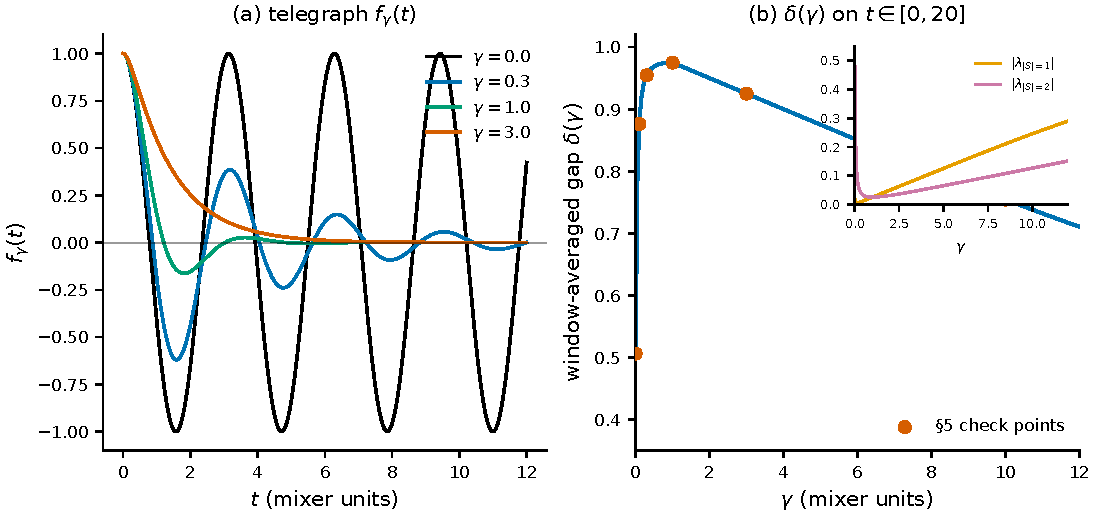
\includegraphics[width=\linewidth]{figures/fig2_solvable_corner.pdf}
\caption{\label{fig:corner}
Solvable corner. (a) Telegraph correlator $f_\gamma(t)$ at
representative $\gamma$. (b) Window-averaged gap $\delta(\gamma)$ on
$t\in[0,20]$, with an inset of the parity-mode eigenvalues
$|\lambda_{|S|=1}|$ versus $|\lambda_{|S|=2}|$. Time-averaging kills the
odd sector; only genuine dephasing kills the even sector. The $n=2$
Lindblad propagator agrees with the formula to $8\times 10^{-16}$.}
\end{figure}

Time randomization and dephasing are both phase randomizers.
Time-averaging kills phases only linearly (odd moments). Coherent
correlations that survive in even moments --- parity observables --- are
killed only by genuine decoherence. Noise \emph{can} help mixing, by
destroying coherent structure that the time window cannot reach.

That interior-optimum phenomenon is not ours. Kendon and
Tregenna~\cite{KendonTregenna2003} found numerically that small
decoherence enhances discrete-time walks on the line, cycle, and
hypercube, with an optimal rate $p\cdot T \approx 2.6$--$5$. Fedichkin,
Solenov, and Tamon~\cite{Fedichkin2006} gave an analytic interior
optimum on cycles. On the hypercube itself, Alagic and
Russell~\cite{AlagicRussell2005} identified a decoherence threshold for
linear instantaneous mixing, and Drezgich
\emph{et al.}~\cite{Drezgich2009} characterized continuous-time mixing
versus Markovian decoherence rate and axis, with an optimal
$\gamma/\Delta \approx 1$--$5$ obtained from the same
non-interacting-qubit factorization used here. Richter~\cite{Richter2007pra,Richter2007njp}
already framed decoherent walks as MCMC, for uniform targets and
without a Metropolis filter. What is new in this corner is the exact
window-averaged telegraph solution, the odd-versus-even-moment
mechanism that separates Layden-style time randomization from genuine
dephasing, and the embedding of that analysis inside an exact MH
sampler. Prior hypercube results concern the walk's own mixing to
uniform.

A finer scan on the e01 chain at $n=4$ reconciles the pilot with the
corner. Interior peaks exist in every cell; their size is controlled by
$\alpha$. At $\alpha=0.3$ and $0.5$ the bumps are $0$--$8\%$ over
$\gamma=0$ --- invisible on G01's coarse grid at $n=6$, so the pilot's
``$12/12$ monotone'' is correct for its cells and is not a law. At
$\alpha=1.0$, in the corner's neighborhood, peaks reach a factor of two
(e.g.\ $T=0.3$: $\delta(0)=0.049\to\delta(0.3\Delta)=0.100$; $T=1.0$:
$0.065\to 0.109$). In all fifteen cells the peak stayed below the best
classical baseline (single-flip gap $0.17$--$0.25$; uniform-flip up to
$0.55$ at high $T$). Noise helped the walk only where the walk was not
worth using.

% Figure 3 is placed here so float numbering stays 1--5 in file order.
% The G01 discussion is in Sec.~\ref{sec:g01}.
\begin{figure*}
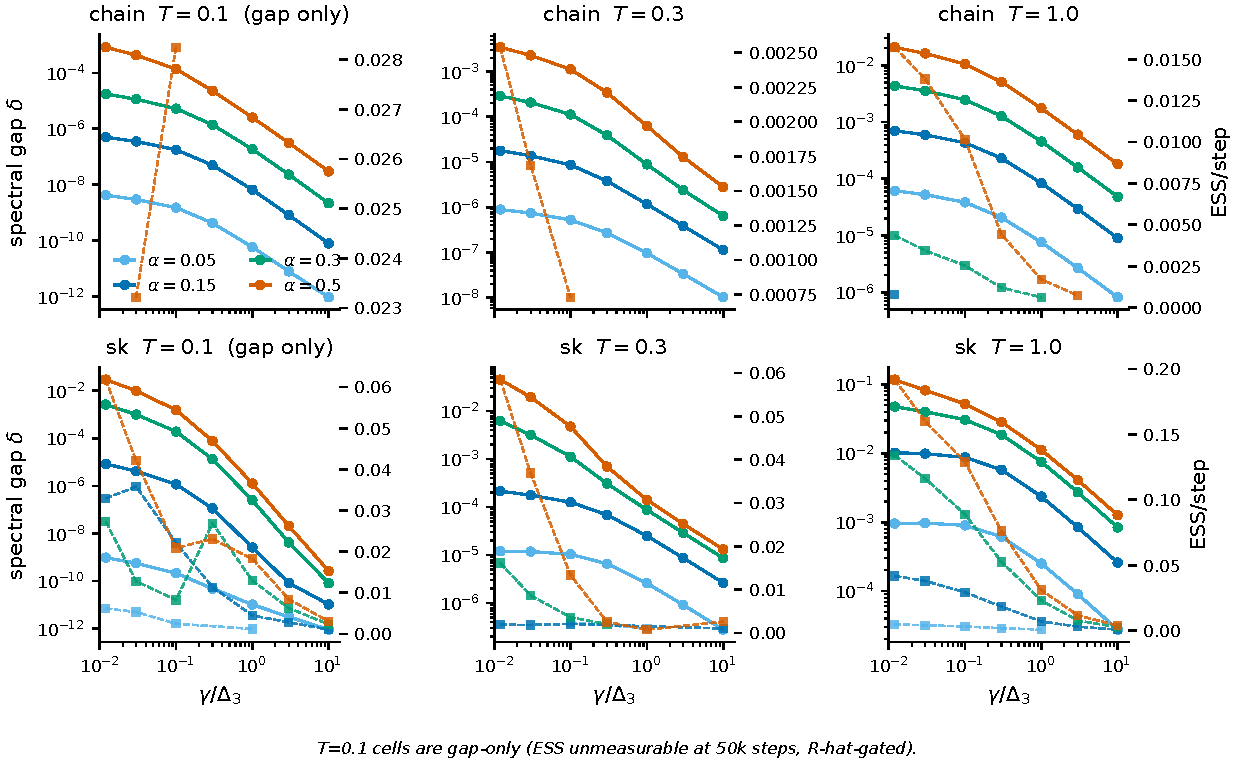
\includegraphics[width=\linewidth]{figures/fig3_g01_scan.pdf}
\caption{\label{fig:g01}
G01 $\gamma$-scan at $n=6$: exact MH gap versus $\gamma$ across
$(T,\alpha)$ cells, with ESS/step overlaid only on $\hat R$-passable
rows. Advantage cells show monotone erosion of the quench. $T=0.1$
cells are gap-only (ESS unmeasurable at $50\,\mathrm{k}$ steps,
$\hat R$-gated).}
\end{figure*}

\subsection{The envelope law}

\noindent\textbf{Envelope law.}
For every target/temperature cell,
\begin{equation}
  \max_{\gamma>0} \delta(\gamma)
  \le
  \max\bigl(\delta(\gamma=0),\; \delta_{\mathrm{SF}},\; \delta_{\mathrm{UF}}\bigr),
\end{equation}
where $\delta_{\mathrm{SF}}$ and $\delta_{\mathrm{UF}}$ are the exact
gaps of Metropolized single-flip and uniform-flip. Equivalently:
wherever the quantum kernel has an advantage, dephasing only erodes it;
wherever dephasing helps, a classical kernel was already better.

The law is not a theorem. A plausible route is that the dephased kernel
lies in the convex hull of phase-kicked quench kernels, and that this
hull's gap envelope is attained on the boundary
$\{\text{coherent quenches}\}\cup\{\text{Zeno/classical limit}\}$. That
convex-hull conjecture is stated, not proved. The paper's evidence is a
pre-registered test, written after the theory pass and before any of the
fifty runs. The registered statement includes a $1\%$ slack
$\varepsilon=0.01$ for propagator discretization; a cell is an L1
violation if its peak exceeds $(1+\varepsilon)$ times the envelope, and
a violation $\ge 5\%$ would have refuted the law.

The test draws fifty cells from a seeded rng (master seed $20260818$):
target class uniform on $\{\text{e01-chain},\,\text{SK},\,\text{RFIM}\}$
with a fresh instance, $n$ uniform on $\{4,5,6\}$, $T$ log-uniform on
$[0.05,10]$, $\alpha$ uniform on $[0.05,1.0]$. The $\gamma$ grid is
$\{0\}\cup\mathrm{logspace}(-2,2,9)$ in units of $\Delta_3$, the
spectral width of $H$. The kernel is the same window-averaged family as
G01 ($t\Delta_3\in[2,12]$, twelve time points). The metric is the exact
MH gap versus the enumerated target.

\noindent\textbf{Result.}
The law holds in $49/50$ cells. One disclosed exception, cell 46, is a
$+1.17\%$ instance-specific micro-bump. Interior peaks occur in $20/50$
cells --- the nuance is generic. Four cells are advantage cells
($\delta(0)$ beats both classical baselines), all of them low-$T$ SK or
RFIM with $\alpha\in[0.63,0.86]$ and $T\in[0.05,0.1]$; in those four,
the $\gamma$-curve is monotone-eroding beyond $\gamma\approx 0.03\Delta$
(sub-$2\%$ instance-specific micro-bumps can occur below that). The
median peak-to-envelope margin is $-72.5\%$. No cell approached the
$5\%$ refutation threshold.

Cell 46 is an SK instance (seed 46), $n=5$, $T=0.085$, $\alpha=0.63$ ---
itself an advantage cell (quench gap $0.0895$ versus single-flip
$1.3\times 10^{-6}$). The curve is $0.0895,\, 0.0906,\, 0.0815,\, 0.0203$
at $\gamma/\Delta_3 = 0,\, 0.01,\, 0.0316,\, 0.1$, peaking at
$\gamma=0.01\Delta_3$ with margin $+1.17\%$ over $\gamma=0$. A finer
$\gamma$ grid maxes at $+1.65\%$ ($\gamma\approx 0.02\Delta_3$, twelve
time points) and survives doubling the time-point count ($+1.2\%$ at
twenty-four points): it is a real property of this instance, not
discretization noise. A fresh SK instance (seed 146) at the identical
$(n,T,\alpha)$ is purely monotone. The bump lives at
$\gamma\sim 0.01$--$0.03\Delta_3$, three orders below the effect H1
needed, and it requires $\gamma$-control precision that makes it useless
as a resource.

\begin{figure}
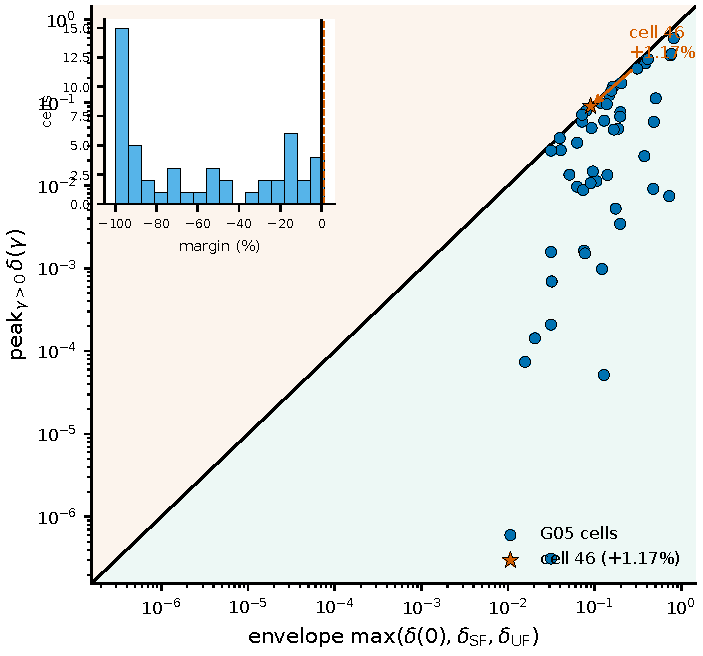
\includegraphics[width=\linewidth]{figures/fig4_envelope.pdf}
\caption{\label{fig:envelope}
Envelope law, fifty pre-registered G05 cells:
$\mathrm{peak}_{\gamma>0}\delta(\gamma)$ versus
$\max(\delta(0),\delta_{\mathrm{SF}},\delta_{\mathrm{UF}})$. The
diagonal is the law boundary. Cell 46 ($+1.17\%$) is marked; the inset
is the margin histogram. Cell 19 is a sub-$\varepsilon$ $+0.087\%$
geometric crossing of the diagonal, not an L1 violation.}
\end{figure}

Orfi and Sels prove that \emph{any} unital quantum proposal ---
dephasing included --- has no speedup over classical sampling on their
marked-item worst case~\cite{OrfiSels2024}. That bound already covers
our whole dephased family on their adversarial instance, against the
uniform baseline. The envelope law is complementary: per-instance,
family-wide, quantitative, on typical Ising/SK/RFIM cells, against the
full baseline envelope, with $\gamma$-resolved erosion. Theirs is
worst-case impossibility; ours is a typical-instance accounting.

\subsection{Advantage cells: the G01 picture}
\label{sec:g01}

The four G05 advantage cells are small-$n$ and sparse. The advantage
\emph{regime} --- low $T$, a coherent quench that already beats
single-flip, $\alpha\le 0.5$ --- is the G01 pilot: $n=6$, e01-chain and
SK, $T\in\{0.1,0.3,1.0\}$, $\alpha\in\{0.05,0.15,0.3,0.5\}$, window
$t\Delta\in[2,12]$, exact gap versus
$\gamma/\Delta_3\in\{0,0.03,0.1,0.3,1,3,10\}$. All twelve cells are
monotone decreasing in $\gamma$. The E01-type quantum advantage over
single-flip persists at low $T$ and is strictly eroded by dephasing; at
$T=1$ the dephased walk falls below the classical baseline by
$\gamma\approx 0.1\Delta$. Representative gaps: chain $T=0.1$,
$\alpha=0.5$ goes
$8.3\times 10^{-4}\to 1.4\times 10^{-4}\to 2.5\times 10^{-6}$ from
$\gamma=0$ to $0.1\Delta$ to $\Delta$, against single-flip
$3.9\times 10^{-9}$; SK $T=0.3$, $\alpha=0.5$ goes
$4.5\times 10^{-2}\to 4.7\times 10^{-3}\to 1.4\times 10^{-4}$, against
single-flip $4.9\times 10^{-4}$.

An ESS confirmation over the pilot's twenty-four $(T,\alpha)$ cells
(both targets; $50\,\mathrm{k}$ steps $\times$ five seeds;
split-$\hat R\le 1.05$ gating) agrees with the gap ordering wherever it
is measurable. Of $216$ kernel-cells, $92$ are $\hat R$-gated --- frozen
or near-frozen chains at large $\gamma$, and the slow chains at
$T=0.1$. Of the fourteen cells with at least three non-gated $\gamma$
points, Spearman $\rho(\mathrm{gap},\,\mathrm{ESS/step})>0.8$ in twelve
and equals $1.0$ in nine. Zero cells show an interior ESS peak. No
$\gamma>0$ beats $\max(\gamma=0,\,\text{classical})$ on ESS/step or
ESS/sec. The one automated flag is a known advantage cell in which the
\emph{walk family} beats uniform-flip, as it should; within the family,
ESS differences across $\gamma\in\{0,0.03,0.1\}$ lie inside one standard
error. Figure~\ref{fig:g01} is the $\gamma$-scan: $T=0.1$ cells are
gap-only.

Peaks are common ($20/50$ in G05; every $n=4$ cell at fine resolution;
the solvable corner). Useful peaks are nonexistent. In advantage cells,
dephasing erodes the advantage beyond $\gamma\approx 0.03\Delta$. That
is the second pillar, in the form a referee can try to break.

\section{Why ENAQT does not transfer to sampling}
\label{sec:mechanism}

The solvable corner and the G05 peak rate ($20/50$) show that the ENAQT
intuition is not wrong about the \emph{walk}. It is wrong about the
\emph{sampler}. The two problems have different objective functions, and
the difference is the Metropolis filter.

ENAQT asks for transport to a sink. There is no quality control: every
amplitude that arrives counts, whether or not it changed the energy. A
little dephasing breaks destructive-interference traps, opens dark
pathways, and raises the arrival probability; too much dephasing
Zeno-freezes the excitation. The Goldilocks peak is a peak in unfiltered
throughput.

MH asks for samples from $\pi \propto e^{-E/T}$. The accept/reject step
prices every proposal by its energy change. At low $T$ the filter
accepts, essentially, only near-degenerate moves. The coherent quench is
valuable \emph{because} its interference concentrates proposal mass on
those near-degenerate pairs --- the same energy-conserving structure
that makes Layden's $\gamma=0$ kernel beat single-flip by many orders of
magnitude on a cold Ising chain. Dephasing is a phase randomizer. It
delocalizes, which is the ENAQT benefit, and it broadens the proposal's
energy distribution, which is an MH cost. The filter then rejects the
spread. Figure~\ref{fig:energy} (Sec.~\ref{sec:outlook}) is a cartoon of
that accounting: a narrow proposal-$\Delta E$ peak sitting inside the
Metropolis window at $\gamma=0$, and a broadened peak spilling out of
the window at $\gamma>0$.

The quantitative handle is already in Sec.~\ref{sec:advantage}. In every
G01 advantage cell the delocalization gain never outruns the acceptance
cost: the gap is monotone decreasing in $\gamma$, the quench advantage
is eroded beyond $\gamma\approx 0.03\Delta$, and at $T=1$ the dephased
walk has fallen below the classical baseline by $\gamma\approx 0.1\Delta$.
The pattern is the same in the four G05 advantage cells. The $\alpha=1$
solvable corner is the complementary check. There the classical energy
$E$ is flat, $\pi$ is uniform, and every proposal is energy-preserving.
The Metropolis filter is idle. Noise is then free to help the walk's own
mixing --- and it does, $0.5\to 0.97$ --- but uniform-flip already has
gap $1$, so the peak is sub-classical by construction. Where the filter
is off, ENAQT wins the walk-versus-walk comparison and loses the
kernel-versus-envelope comparison. Where the filter is on, ENAQT loses
both.

Two distinctions keep the bookkeeping honest. First, time-averaging is
also a phase randomizer, but it is not a substitute for dephasing. The
window kills odd moments and leaves even-moment (parity) coherences;
only genuine noise kills those (Sec.~\ref{sec:advantage}).
Time-averaging does \emph{not} smear energy on a given realization ---
each trajectory still evolves under a real Hamiltonian --- so it does
not pay the MH penalty that dephasing pays. Second, the walk
literature's noise-beats-classical results compare a decohered walk to
the classical walk on the same sparse graph, toward a uniform target,
with no acceptance filter. That is a different contest than the one the
envelope law runs. The Metropolis filter is precisely what flips the
verdict: walk-versus-walk, uniform target, no filter, and noise can win;
kernel-versus-envelope, Gibbs target, MH filter, and noise never does.

Nothing in this section is a design rule for future kernels. The
observations fit a picture in which the quench's value is
energy-conserving interference and dephasing spends that value. Whether
a scalar ``energy concentration'' predicts advantage across kernels and
targets is a conjecture, stated as such in Sec.~\ref{sec:outlook}, and
is not claimed here.

\section{Benchmarking protocol}
\label{sec:protocol}

Quantum-algorithm benchmarks are easy to fool. The rules below are the
instrument, not the appendix. They are the TunnelVision exactness
harness, applied here to a noise-as-resource hypothesis and offered as a
reusable method.

\emph{Exactness boundary.}
Proposal kernels never see target log-probabilities. Nothing quantum
sits on the accept side of MH. A kernel returns a triple
$(y,\, \log q_{\mathrm{fwd}},\, \log q_{\mathrm{rev}})$; for every
transpose-closed channel the two logs are identically zero by
Theorems~\ref{thm:tc} and~\ref{thm:lindblad}, but the interface does not
get to assume that. The G01/G05 runners consume the triple and never a
$\pi$-lookup from the kernel.

\emph{Two clocks.}
Every experiment reports ESS per step \emph{and} ESS per second. A
kernel that wins per step and loses wall-clock by orders of magnitude is
a negative result at the system level. Spectral gap, where the
$2^n\times 2^n$ kernel can be built, is a third number, not a
substitute.

\emph{Mixing gate.}
Split-$\hat R\le 1.05$ gates a chain before its ESS is believed. The
gate exists because frozen chains produce garbage-high ESS on a
near-constant series --- the pathology that appeared in G05 at
$\gamma=31.6\Delta$ and in $92$ of $216$ G01 kernel-cells. Those cells
are excluded, not averaged away.

\emph{Enumerated truth.}
At $n$ small enough to enumerate, we report error against the exact
$\pi$ (and the exact gap) rather than against a surrogate. No
translation layer: the walk graph \emph{is} the spin system.

\emph{Pre-registration.}
Kill criteria are written before data. G01's H1 rule --- an interior
$\gamma$ must beat both $\gamma=0$ and the largest $\gamma$ outside
$\pm 2$ SE --- was fixed in the runner. G05's envelope law, the $1\%$
slack, the $5\%$ refutation threshold, and the ``holds with noted
exceptions'' band for one or two sub-$5\%$ violations were fixed in the
pre-registration before the fifty-cell runner existed. The originally
tempting law (monotone gap for all targets) was \emph{not} registered:
the theory pass had already refuted it, and pre-registering a
known-false claim would have been theater.

\emph{Negatives at full strength.}
A failed hypothesis is a result. H1 is reported as killed, not as ``more
work needed.'' Cell 46 is reported in full, not absorbed into a mean.
The un-$\sqrt{\phantom{x}}$ stationary bound is flagged as empirical.
The interior-optimum mixing phenomenon is cited as known
(Sec.~\ref{sec:related}); we claim only the analysis we own.

The protocol earned its keep twice. It killed H1 on the G01 pilot:
twelve of twelve cells monotone in the gap, zero ESS peaks under
$\hat R$ gating, envelope intact on both clocks. It then caught the
overreach of conjecture v1. The theory pass produced interior peaks at
$\alpha=1$ and on a fine $n=4$ grid; registering monotonicity at that
point would have been a pre-registered falsehood. The corrected,
pre-registered claim is the envelope law, tested on fifty cells the
theory pass had never seen. That sequence --- kill fast, then refuse to
promote a refuted conjecture --- is the method contribution. H2 and H3
are moot as stated: no useful $\gamma^\ast$ exists, so a
matching-condition study and a hardware-idle test do not proceed.

\section{Outlook: energy concentration as a predictor}
\label{sec:outlook}

The observations of Secs.~\ref{sec:advantage} and~\ref{sec:mechanism}
fit a single accounting: the quench is valuable when its proposals sit
on near-degenerate pairs, and dephasing spends that value by broadening
proposal energy. We record that accounting as a conjecture, not as a
theorem of this paper.

\noindent\textbf{Conjecture (energy concentration).}
The advantage of a proposal $q$ over trivial classical kernels is
predicted by the proposal mass on near-degenerate pairs,
\begin{equation}
  C(q)
  =
  \sum_{x,y} \pi(x)\, q(y|x)\, \mathbf{1}\bigl[\,|E(y)-E(x)| \le \kappa T\,\bigr],
\end{equation}
for an $O(1)$ window $\kappa$. Kernels should be engineered for energy
concentration, not for delocalization.

Everything already measured is consistent with $C(q)$ and does not prove
it. Dephasing lowers $C$ (broadened proposal energy) and erodes
advantage (G01, G05 L2(b)). Time-averaging preserves $C$, because energy
conservation is per-realization of a real Hamiltonian, and does not
erode advantage the way dephasing does. The $\alpha=1$ corner has flat
$E$, so $C$ is identically $1$ and noise can only help sub-classically
--- which is what the telegraph solution shows. Figure~\ref{fig:energy}
is the cartoon of that split, not a fit to data.

\begin{figure}
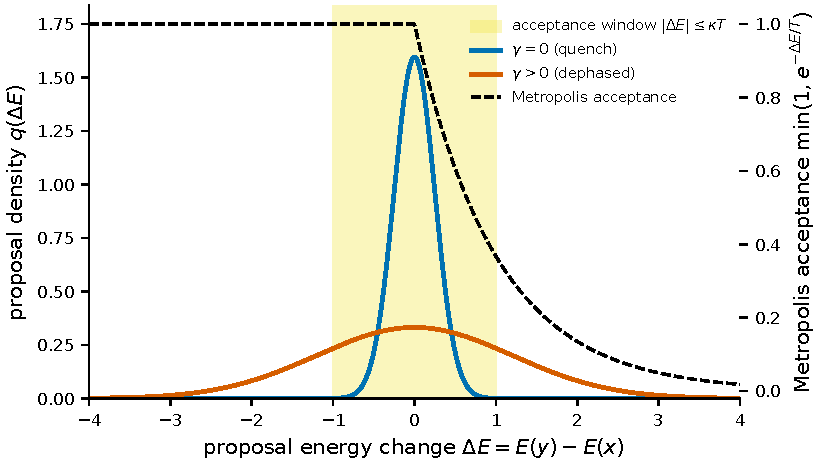
\includegraphics[width=\linewidth]{figures/fig5_energy_concentration.pdf}
\caption{\label{fig:energy}
Proposal energy change $\Delta E = E(y)-E(x)$ at $\gamma=0$ (narrow,
sitting inside the Metropolis window) versus $\gamma>0$ (broadened,
spilling out of the window). The overlaid curve is the Metropolis
acceptance $\min(1,e^{-\Delta E/T})$. Energy concentration $C(q)$ is a
proposed predictor of advantage, not a theorem of this paper.}
\end{figure}

A next-project test is direct: compute $C(q)$ for the quench, the
dephased family, single-flip, and uniform-flip across a draw of
targets, and regress measured ESS (or gap) advantage on $C$. If the
regression is tight, $C$ becomes a design objective. If it is not, the
mechanism of Sec.~\ref{sec:mechanism} is still the right qualitative
story and the scalar is the wrong summary.

Three escapes from G01 were not pursued, and we do not want them read as
hidden rescues of H1. Site-dependent rates $\gamma_i$ could \emph{shape}
where proposals land rather than how coherent they are. Noise in the
basis of a frustrated subspace, rather than the computational basis, is
a different channel, still transpose-closed if the jumps are
real-symmetric (Theorem~\ref{thm:tc}) but not the family G01/G05
scanned. Hitting-time objectives --- first arrival at a ground-state
set --- restore a sink, and are optimization, not sampling. Each is a
new hypothesis. None of them, if true, would change
Theorems~\ref{thm:tc}--\ref{thm:stationary} or the envelope law as
stated for uniform computational-basis dephasing inside exact MH.

\section{Related work}
\label{sec:related}

We group neighbors in the order a reader should meet them: the
decohered-walk mixing literature that already owns the interior-optimum
phenomenon; the quantum-enhanced MCMC line we sit on; and ENAQT, whose
objective we do not share.

\subsection{Decohered-walk mixing --- the known phenomenon}

Fastest mixing at intermediate decoherence is established walk
literature, including on the hypercube that is our $\alpha=1$ graph.

Kendon and Tregenna~\cite{KendonTregenna2003} showed numerically that
small decoherence enhances discrete-time walks on the line, cycle, and
hypercube, with an optimal rate $p\cdot T \approx 2.6$--$5$ and a mixing
time on the cycle below the classical value. Fedichkin, Solenov, and
Tamon~\cite{Fedichkin2006} gave the analytic counterpart on cycles:
mixing time improves linearly in the decoherence rate at small rates,
degrades linearly at large rates, and has a unique interior optimum.
Abal \emph{et al.}~\cite{Abal2007} found a mixing-time minimum at
broken-link probability $p\approx 0.1$ for a discrete-time hypercube
walk.

On the continuous-time hypercube, Alagic and
Russell~\cite{AlagicRussell2005} identified a decoherence threshold
below which linear instantaneous mixing survives, with classical
$\Theta(n\log n)$ behavior and Zeno retardation beyond it. Drezgich
\emph{et al.}~\cite{Drezgich2009} gave a complete characterization
versus Markovian decoherence rate \emph{and} axis: a finite optimal rate
$\gamma/\Delta \approx 1$--$5$ for almost all decoherence axes (none for
axes in the $x$--$y$ plane), derived from the same
non-interacting-qubit factorization our telegraph solution uses. Those
results are fixed-$t$ instantaneous mixing to uniform; they have no
window average, no Metropolis filter, and no classical-envelope
comparison.

Richter~\cite{Richter2007pra,Richter2007njp} is the closest in spirit:
decoherent walks always mix; mixing is robust to any smooth decoherence;
the framing is already MCMC/sampling; threshold mixing is proved for the
hypercube $\mathbb{Z}_2^n$; a $\sqrt{\delta}$ quantum speedup of
classical mixing is conjectured. The target is uniform; decoherence is
repeated measurement; there is no Metropolis filter, no Gibbs target,
and no noise-rate optimization against a classical-kernel envelope.

The quantum-stochastic-walk umbrella~\cite{Whitfield2010} and the
transport-optimal $90\%$/$10\%$ quantum/classical mixture of Caruso
\emph{et al.}~\cite{Caruso2014} belong here as framework, but the latter
optimizes transport to a sink, not mixing.

We cite this group first and prominently because it is the phenomenon
behind our solvable corner. Our claim in that corner is the
window-averaged telegraph solution, the odd/even-moment mechanism, and
the exact-MH embedding --- not the existence of an interior mixing
optimum.

\subsection{Quantum-enhanced MCMC}

Layden \emph{et al.}~\cite{Layden2023} is the $\gamma=0$ limit of our
kernel: coherent quench proposals, exact MH, noise treated as a
nuisance. Their Supplemental Material already states the convergence
condition we formalize --- errors are harmless provided they do not
break $Q(s'|s)=Q(s|s')$ symmetry on average --- with SPAM-twirling
mitigation, and notes that depolarizing noise degrades the proposal
toward uniform. Theorems~\ref{thm:tc} and~\ref{thm:lindblad} are the
systematic channel-level classification of which physical noise
satisfies that condition (transpose-closed Kraus, unitality, $T_1$ as
the unique realistic bias channel). That is a strictly stronger
statement, and not a bolt from the blue.

Orfi and Sels~\cite{OrfiSels2024} prove that \emph{any} unital quantum
proposal has no speedup over classical sampling on their marked-item
worst case. Dephasing is unital, so their bound covers our whole
dephased family on that adversarial instance, against the uniform
baseline. The envelope law is complementary: per-cell, pre-registered,
quantitative, on typical Ising/SK/RFIM instances, against the full
baseline envelope, with $\gamma$-resolved erosion. We cite them as a
sibling, not as a special case of us or the reverse.

Follow-ups in the qe-MCMC line have not studied tuned noise.
Coarse-grained qe-MCMC~\cite{Ferguson2025} says explicitly that the
effect of noise ``has not been investigated.'' The quantum-inspired
surrogate of Christmann \emph{et al.}~\cite{Christmann2024} repeats the
noise-affects-only-efficiency point without a $\gamma$ scan. The
causal-set application~\cite{Ferguson2025causal} has no noise angle.

Fault-tolerant Metropolis walks are a different machine model: the walk
\emph{is} the chain, not a noisy proposal inside classical MH. We cite
Lemieux \emph{et al.}~\cite{Lemieux2020}, Claudon
\emph{et al.}~\cite{Claudon2025}, penalised qubitized
walks~\cite{CarrascoArango2026}, and Incudini and
Mazzola~\cite{IncudiniMazzola2026} in passing.

Dissipative Gibbs samplers~\cite{Zhang2023,Chen2023} engineer a
Lindbladian whose fixed point \emph{is} the Gibbs state. That is
constructive dissipation, not ambient tuned dephasing inside an exact
MH proposal.

\subsection{ENAQT and device-noise sampling}

Rebentrost \emph{et al.}~\cite{Rebentrost2009} and Lloyd and
Mohseni~\cite{LloydMohseni2011} are the transport Goldilocks; their
citation trees stay in photosynthesis and exciton transport. Digital
ENAQT~\cite{Gallina2022,Gallina2024} supplies the circuit unravellings
we reuse (stochastic-Hamiltonian phase kicks; collision scheme). Those
works target transport simulation; they note that converting intrinsic
device noise into a programmable stochastic process has not been
achieved. D-Wave device-noise sampling~\cite{Nelson2022} is analog and
biased, with no exactness layer.

\subsection{Positioning}

What is ours: the first channel-level exactness characterization for
noisy walk proposals, upgrading Layden's SM condition to a
classification; the first study of decohered-walk \emph{mixing} results
embedded in an exact MH sampler with Gibbs targets; and the envelope law
as the negative answer to noise-as-resource for \emph{sampling}. The
interior-optimum mixing phenomenon itself is 2003--2009 walk literature
and is cited as such. The Metropolis filter is what separates the
verdicts. Walk-versus-walk, uniform target, no filter: noise can win.
Kernel-versus-envelope, Gibbs target, MH filter: noise never wins.

\begin{acknowledgments}
TODO: acknowledgments.
\end{acknowledgments}

\section*{Data availability}

The certification scripts, figure generators, pre-registration, and
numerical results that support the claims of this paper are included
with the manuscript source: the R1 and $T_1$-bias runners and tests
I10--I13; the figure generators under \texttt{paper/figures/}; the G05
pre-registration, \texttt{results.csv}, and verdict; the G01 ESS
confirmation table; and the certified R1 and amplitude-damping result
files. A public archival deposit will be made at submission
(TODO: ZENODO-DOI).

\bibliography{refs}

\end{document}
